%*****************************************************************************************
%*********************************** Third Chapter **************************************
%*****************************************************************************************

\chapter{Plasmonic nanostructures}

\graphicspath{{Chapter3/Figures/}}

\section{Introduction}
Surface plasmons are collective electron oscillations in a metal. The form of such oscillations can be found by solving Maxwell's equations, and depends on the geometry of the problem. Such movement of electrons causes large field enhancement, and the resonance frequency is very sensitive to the dielectric environment around the metal. In this Chapter we will solve Maxwell's equations to find the form of plasmon oscillations at a metal-dielctric interface, before exploring how the solution is affected by modifying the metal surface to form a grating. Finally we will explore plasmon oscilltions in small metal islands.

\section{Surface plasmon polaritons}
In order to describe the behaviour of electrons in a metal, we can use Maxwell's equations to describe the behaviour of electromagnetic fields:
\begin{subequations}
\label{Maxwell}
\begin{align}
\nabla \cdot \vec{D} &= \rho \label{Maxwell1}\\
\nabla \cdot \vec{B} &= 0 \label{Maxwell2}\\
\nabla \times \vec{E} &= - \frac{\partial \vec{B}}{\partial t} \label{Maxwell3}\\
\nabla \times \vec{H} &= \vec{J} + \frac{\partial \vec{D}}{\partial t} \label{Maxwell4}. 
\end{align}
\end{subequations}
These equations link the fields $\vec{D}$ (dielectric displacement), $\vec{E}$ (electric field), $\vec{H}$ (magnetic field) and $\vec{B}$ (magnetic flux density). The electric charge density is given by $\rho$, and electric current density by $\vec{J}$. For linear, isotropic and non-magnetic materials we have the relationships
\begin{subequations}
\label{fieldrelations}
\begin{align}
\vec{D} &= \epsilon \epsilon_0 \vec{E} \label{DE}\\
\vec{B} &= \mu \mu_0 \vec{H} \label{BH},
\end{align}
\end{subequations}
where $\epsilon_0, \mu_0$ are the permittivity and permeability of free space respectively, and $\epsilon, \mu$ are the relative permittivity and permeability of the material in question. In the case of a non-magnetic medium $\mu=1$, and the refractive index $n$ is given by $\sqrt{\epsilon}$.

By combining Eqs.\,(\ref{Maxwell3}, \ref{Maxwell4}) and assuming a harmonic time dependence to the electric field with frequency $\omega$ such that $\vec{E}(\vec{r},t) = \vec{E}(\vec{r})e^{-i\omega t}$, we find the Helmholtz equation
\begin{equation}
\centering
\nabla^2\vec{E} + k_0^2\epsilon \vec{E} = 0,
\label{Helmholz}
\end{equation}
where $k_0 = \frac{\omega}{c}$ is the wavevector of the wave in vacuum.
\begin{figure}[ht] 
\centering    
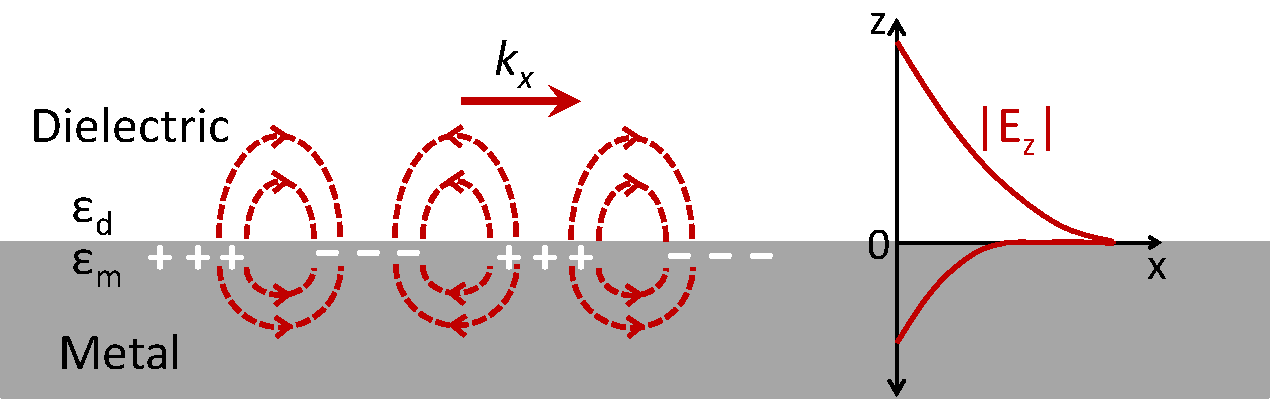
\includegraphics[width=0.8\textwidth]{Fig1}
\caption{Schematic for SPP oscillations at a metal-dielectric surface, showing the evanescent nature of such plasmons.}
\label{3Fig1}
\end{figure}

Using the geometry of a metal-dielectric interface shown in Fig.\,\ref{3Fig1}, we look for solutions of waves propagation in the $x$ direction but confined to the interface with evanescent decay in the $z$ direction, such that $\vec{E}(x,y,z,)=\vec{E}(z) e^{i k_x x}$ where $k_x$ is the propagation constant of the wave. We find one set of solutions that is transverse electric (TE) polarised, with teh $\vec{E}$-field component perpendicular to the direction of travel:
\begin{subequations}
\label{TEplasmons}
\begin{align}
H_x &= i \frac{1}{\omega \mu_0} \frac{\partial E_y}{\partial z}\\
H_z &= \frac{k_x}{\omega \mu_0} E_y\\
\frac{\partial^2 E_y}{\partial z^2} &+ (k_0^2 \epsilon_i-k_x^2)E_y = 0 .
\end{align}
\end{subequation}
For both solution the subscript $i$ refers to the material the wave is travelling in, $d$ or $m$ for the dielectric and metal respectively. The solutions are waves of the form $e^{i k_x x} e^{k_i z}$, i.\,e.\, a wave travelling in x direction that evanescently decays in the z direction. Applying the boundary conditions of $E_y$ and $H_x$ continuity across the metal-dielectric interface, we find the condition 
\begin{equation}
\centering
A(k_m+k_d)=0 ,
\label{TEcont}
\end{equation}
where $A$ is the amplitude of wave in the metal halfspace. Since confinement requires Re$(k_m, k_d)>0$, Eq.\,\ref{TEcont} is only fulfilled if $A=0$ when no wave can be sustained in the metal. The boundary condition indicate similarly the amplitude of the wave must be 0 in the dielectric as well, thus no SPPs exist in TE polarisation.

The transverse magnetic (TM) polarised solution, with the $\vec{H}$-field component perpendicular to the direction of travel, is:
\begin{subequations}
\label{TMplasmons}
\begin{align}
E_x &= -i \frac{1}{\omega \epsilon_i \epsilon_0} \frac{\partial H_y}{\partial z}\\
E_z &= -\frac{k_x}{\omega \epsilon_i \epsilon_0} H_y\\
\frac{\partial^2 H_y}{\partial z^2} &+ (k_0^2 \epsilon_i-k_x^2)H_y = 0 \label{TMwave}.
\end{align}
\end{subequation}
Here continuity of $H_y$ and $\epsilon_i E_z$ across the interface requires
\begin{equation}
\centering
\frac{k_d}{k_m} = -\frac{\epsilon_2}{\epsilon_1} ,
\label{TMcont}
\end{equation}
so we require Re[$\epsilon_1$] and $\epsilon_2$ to be of opposite signs, thus SPPs can only be sustained on a metal-insulator interface. Fulfillment of Eq.\,\ref{TMwave} leads to 
\begin{subequations}
\label{k_relations}
\begin{align}
k_m^2 &= k_x^2-k_0^2\epsilon_m\\
k_d^2 &= k_x^2-k_0^2\epsilon_d .
\end{align}
\end{subequations}
Combining this with Eq.\,\ref{TMcont} produces
\begin{equation}
\centering
k_x = k_0\sqrt{\frac{\epsilon_m \epsilon_d}{\epsilon_m + \epsilon_d}} ,
\label{SPPdispersion}
\end{equation}
the dispersion relation of an SPP on a metal-dielectric interface. Fig.\,\ref{3Fig2}(a) shows the calculated dispersion using a free electron gas model for the metal-air SPP, with values taken from Ref.\,\cite{Zeman1987}). In this model there is no damping in the metal, i.\,e.\,Im($\epsilon_m)=0$. Note three regions in the graph: at high frequencies above the plasma frequency of the electron gas $\omega_p$ we have the transparent region ($k_x, k_i$ real) where radiation can penetrate into the metal and excite plasmon polaritons. At low frequencies we have bound surface modes ($k_x$ real, $k_i$ imaginary), and at large $k_x$ the frequency tends to $\omega_{sp} = \frac{\omega_p}{1+\epsilon_d}$. In this limit the plasmons are stationary surface plasmons, and $\epsilon_m+\epsilon_d=0$. For $\omega_{sp}<\omega<\omega_p$ no propagating modes exist ($k_x$ imaginary). If damping is included in the metal model, then quasi-bound modes can exist in this intermediate region [Fig.\,\ref{3Fig2}(b), calculated using values for Ag from ?]. Note also damping introduced a finite maximum $k_x$ for the SPP, leading to a finite propagation length $L_x = \frac{1}{2\textnormal{Im}(k_x}$, typically on the order 10-100\,$\mu$m at visible wavelengths for Au/Ag \cite{Maier2007}. The limit in $k_x$ also produces an upper limit in $k_i$ [Eq.\,\ref{k_relations}], thus limiting the skin depth $L_z = \frac{1}{\textnormal{Im}(k_i}$ to order 10\,nm in metals. 
\begin{figure}[ht] 
\centering    
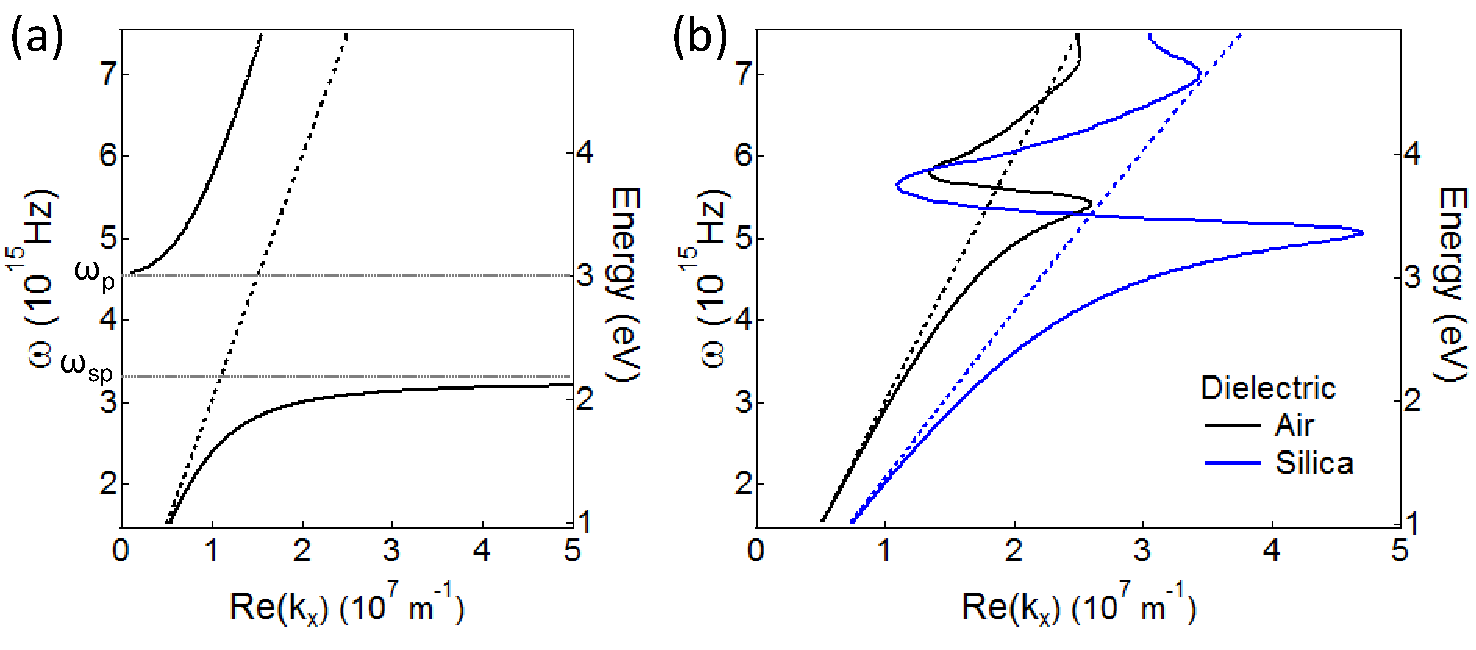
\includegraphics[width=0.8\textwidth]{Fig2}
\caption{Dispersion of SPPs on metal-dielectric interface for (a) free electron gas and (b) silver (solid lines), and light lines in the dielectric (dashed lines).}
\label{3Fig2}
\end{figure}


\section{Plasmonic gratings}
\label{sec:plasmonicgratings}
From Fig.\,\ref{3Fig2} we can see that the SPP dispersion always lies on the right of the light line in the dielectric, and this momentum mismatch means that it is not possible to directly excite SPPs using photons. Instead we must use a phase matching technique, for example prism or grating coupling. In prism coupling a three-layer system is employed, so that photons reflected at the higher refractive index interface has sufficient momentum to excite SPPs on the interface between the metal and the lower refractive index material. In grating coupling, due to its periodicity $D$ the grating structure can provide momenta of $G_m = \frac{2\pi m}{D}$, thereby allowing photons to couple to SPPs. However other types of modes can be observed in the optical spectra of plasmonic gratings.

\subsection{First order modes}
Using Huygens' construction and considering each point on the grating as a wave scatterer, we reach the well-known grating equation for constructive interference
\begin{equation}
\centering
D(\sin\alpha-\sin\beta) = l\lambda ,
\label{GratingEq}
\end{equation}
where $\alpha$ is the angle of incidence and $\beta$ the diffracted angle with respect to the grating normal, $\lambda$ is the wavelength of light and $l$ the order of the diffracted light [Fig.\,\ref{3Fig3}(a)]. From here we only consider the zeroth diffraction order (i.\,e.\, specular reflection) with incidence angle $\theta$ and azimuthal angle $\phi$. In the order approximation, where we assume different types of diffracted light do not interact, we can distinguish between two types of gratings modes: `photonic' modes caused purely by interference of light due to the periodic structure, and `plasmonic' modes where SPPs are excited on the surface of the grating. We can find the dispersion of such grating modes by considering momentum and energy conservation of incoming/outgoing photons, and thus find
\begin{equation}
\centering
k_m = k_i^2\sin^2\theta+G_m^2\pm2k_iG_m\sin\theta\cos\phi ,
\label{GratingDisp}
\end{equation}
where the label $m$ indicates the order of grating vector $G_m$ needed for matching. Here the wavevector of the incident light
\begin{subequations}
\label{kmodes}
\begin{equation}
\centering
k_i = \frac{\omega}{c}\sqrt{\epsilon_d} ,
\label{ki}
\end{equation}
for photons
\begin{equation}
\centering
k_m=\frac{\omega}{c} ,
\label{kphot}
\end{equation}
and for SPPs
\begin{equation}
\centering
k_m = \frac{\omega}{c}\sqrt{\frac{\epsilon_m\epsilon_d}{\epsilon_m+\epsilon_d}} .
\label{kspp}
\end{equation}
\end{subequations}
In this case the grating can be thought of as a 1D photonic grating, where the photon/SPP dispersions are displaced by multiples of the grating vector. Although in the first order photonic and plasmonic modes do not interact with each other, SPP modes can strongly couple and create anticrossings in the spectra \cite{Chen1983}.
\begin{figure}[ht] 
\centering    
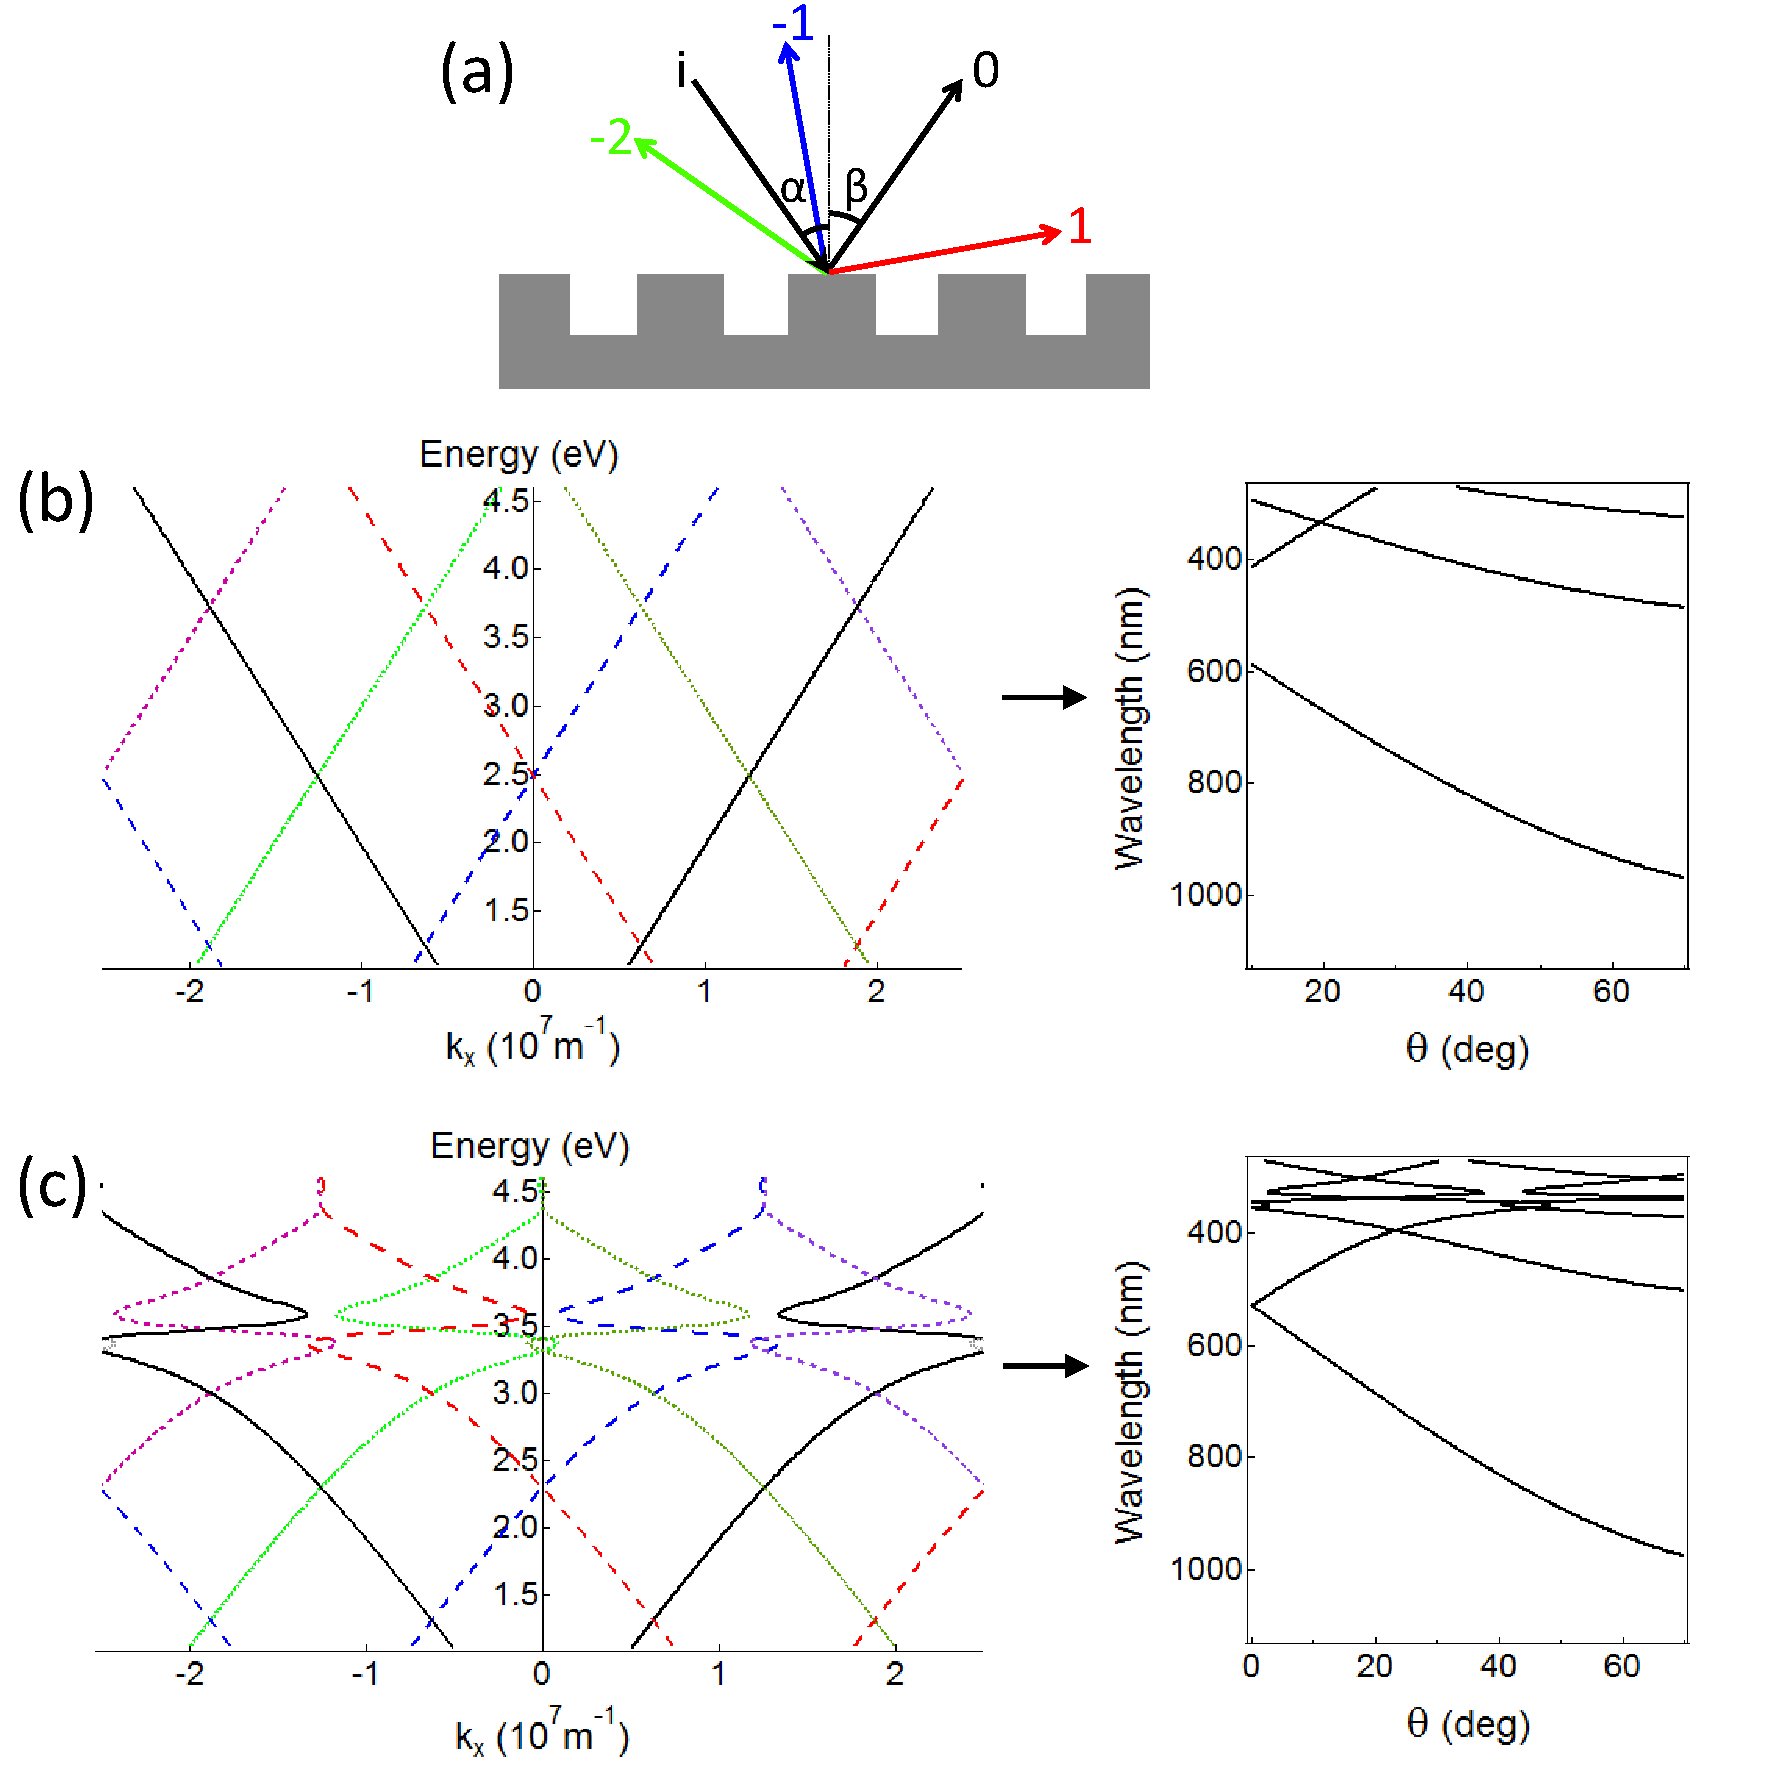
\includegraphics[width=0.8\textwidth]{Fig3}
\caption{(a) Diffraction from a 1D grating structure, showing the incident light and diffracted orders. Dispersion (left) and modes as a function of incidence angle $\theta$ (right) for (b) photonic and (c) plasmonic modes for specularly reflected zeroth order mode for a $D=500$\,nm grating.}
\label{3Fig3}
\end{figure}


\subsection{Grating anomalies}
Anomalies are sharp changes in the response of a grating, and first observed by Wood, who noted ``that under certain conditions the drop from maximum illumination to maximum...occurred within a range of wave-lengths not greater than the distance between sodium lines" \cite{Wood1902}. Anomalies are second order effects, where different diffracted modes interact with each other. The effect is named after Wood, and in plasmonic gratings occurs as a sharp increase in intensity followed by a dip [Fig.\,\ref{3Fig4}]. Although overall the Wood's anomaly is one physical phenomenon, it is possible to separate into two parts for a more intuitive understanding: the threshold (sharp change in intensity) and resonance (dip) anomalies.
\begin{figure}[ht] 
\centering    
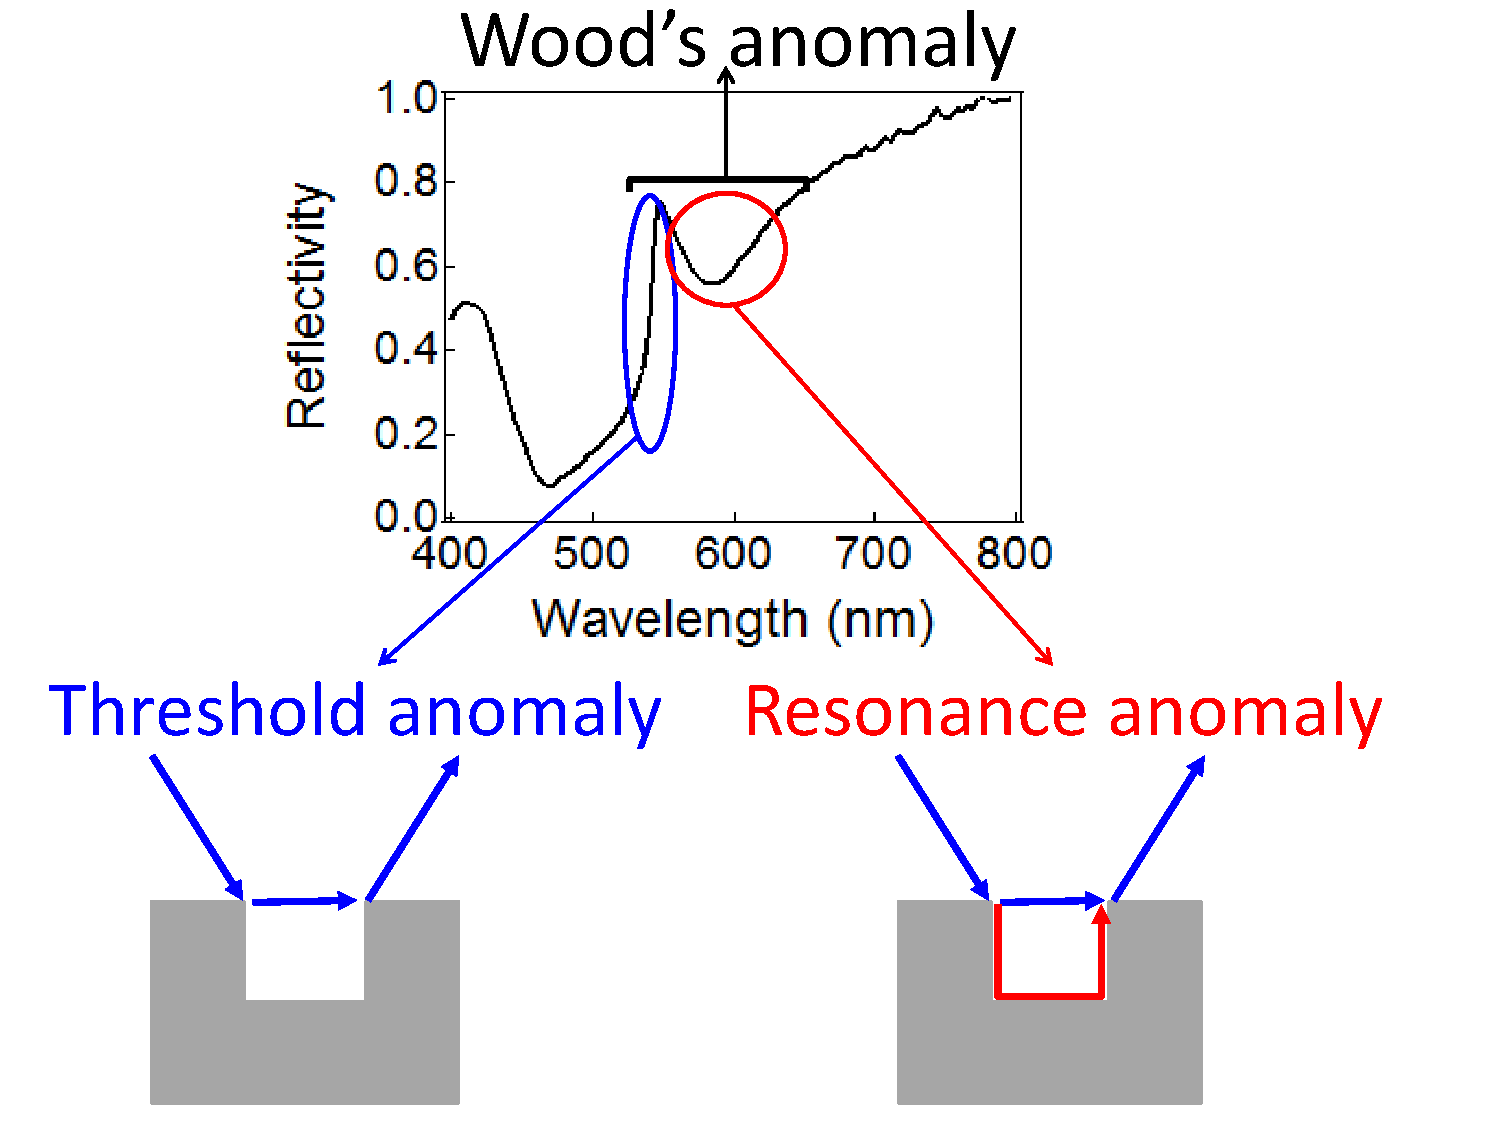
\includegraphics[width=0.6\textwidth]{Fig4}
\caption{Wood's anomaly in the reflectivity of Ag grating, $D=417$\,nm. Schematics of the threshold and resonance anomalies are included. }
\label{3Fig4}
\end{figure}

The threshold anomaly is a photonic effect, and comes about when an order is diffracted along the surface of the grating ($\beta=90^{\circ}$). If an order becomes evanescent then the energy available will be redistributed to the other diffractive orders, thus this `passing' order on the edge between diffraction and evanescence leads to a sharp change in the diffraction intensity. These effects are still due to interference from grating structure, and thus occur at the predicted first order photonic modes [Eq.\,\ref{GratingEq}]. The threshold anomaly can be observed in both polarisation, but generally the strength of the anomaly (i.\,e.\,the change from maximum to minimum intensity) is smaller in TE polarisation, particularly in metals, as the $E$-field is parallel to the grating lines in this case and thus cannot be sustained. The reduction in field intensity leads to less energy to redistribute, hence the effect is less pronounced. 

The resonance anomaly is a plasmonic effect, and comes from the excitation of surface waves on the grating. The excited SPPs can interact with the diffractive light, and the addition of the SPP oscillator and background photonic diffracton leads to a Fano resonance, giving the typical peak-trough feature seen. Clearly the resonance anomaly can only be observed when SPPs are excited, e.\,g.\, for $\phi=0^{\cric}$ in TM polarisation, but not TE. Unlike the threshold anomaly, the position and linewidth of the resonance anomaly dip cannot be predicted by Eq.\,\ref{GratingEq} as it depends on the nature of the SPP, and is thus sensitive to the geometry of the grating and any surface roughness in the material [Fig.\,\ref{3Fig5}]. However it is possible to calculate the position of the resonance anomaly by using electromagnetic theory to model the grating (see Refs.\,\cite{Hutley1982, Loewen1997} and references therein). 

Grating anomalies have been observed in both reflection and transmission gratings, and are responsible for the extraordinary transmission observed for some 1D and 2D arrays \cite{Fano1941, Hessel1965, Lee2005, Lochbihler1994, Ritchie1968, Treacy2002, Watts1997}. Overcoating of a metallic grating affects the strengths and positions of anomalies, in particular the resonance anomaly, where the SPP is very sensitive to the local dielectric environment. In addition, light can excite modes in the coating material, and thus change the direction of the $E$-field so that anomalies can be excited when they're not predicted to, e.\,g.\, $\phi=0^{\circ}$ in TE polarisation \cite{Hutley1982, Loewen1997}.
\begin{figure}[ht] 
\centering    
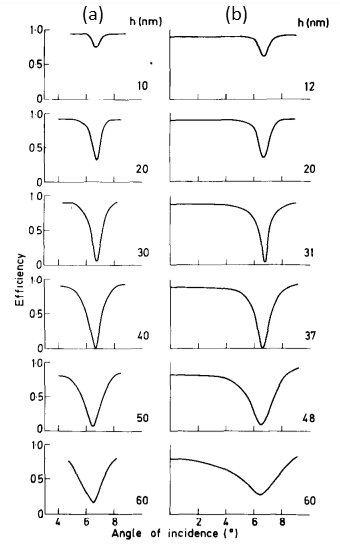
\includegraphics[width=0.5\textwidth]{Fig5}
\caption{Dependence of resonance anomaly on the grating depth $h$ for sinusoidal grating, $D=556$\,nm at $\lambda=647$\,nm from (a) electromagnetic theory and (b) experiment. Reproduced from Ref.\,\cite{Hutley1976}. }
\label{3Fig5}
\end{figure} 

\subsection{Localised and guided modes}
Gratings can also give rise to optical modes that do not rely on the periodicity of the structure. In particular the grating slits can be thought of as independent, sustaining modes that do not couple to modes in nearby slits. We can think of the slits as hollow electromagnetic waveguides, and thus support modes that fit the equation \cite{Jackson1999} [CHECK JACKSON]
\begin{equation}
\centering
\frac{\omega^2}{c^2}(n_{\mathit{eff}}^2-\sin^2\theta) = \pi^2\left(\frac{\mu^2}{a_{\mathit{eff}}^2}+\frac{\nu^2}{b_{\mathit{eff}}^2}\right) ,
\label{waveguide}
\end{equation}
where $n_{\mathit{eff}}$ is the effective refractive index experience by the mode in the grating slit, $a_{\mathit{eff}}$ is the effective width and $b_{\mathit{eff}}$ half the effective height for the mode, and $\mu, \nu$ are indices used to label the waveguide mode. Due to the penetration depth of the electromagnetic field in metals, $a_{\mathit{eff}}$ is not the same as the geometric width of the grating slit, and particularly if there is a coating on the metal then $a_{\mathit{eff}}$ and $b_{\mathit{eff}}$ both have some dependence on $n_{\mathit{eff}}$. 

Surface plasmons travelling down the grating slits can interact, particularly if the slit is narrow. In this case we can form symmetric and antisymmetric combinations of the SPP oscillations, essentially forming a metal/insulator/metal waveguide \cite{Maier2007}. For rectangular shaped slits, often known as trench waveguide, the highest $E$-field intensity is often at the top corners of the slits [Fig.\,\ref{3Fig6}(a)] and thus more extended outside the groove \cite{Bozhevolnyi2005, Srivastava2009, Chattopadhyay2012}. If the groove is V-shaped, the change in effective refractive index due to the change in width leads to reflections, and the highest $E$-field is localised at the bottom of the grooves [Fig.\,\ref{3Fig6}(a)] and such oscillations are called channel plasmon polaritons \cite{Bozhevolnyi2005, Srivastava2009, Novikov2002, Kuttge2009, Sondergaard2012}. Due to their localised nature, the dispersion of such modes is often flat with respect to the angle of incidence $\theta$. Such channel plasmon polaritons can be observed in near-field optical microscopy [Fig.\,\ref{3Fig6}(b)], and show interference with the light scattered by the structure.

\begin{figure}[ht] 
\centering    
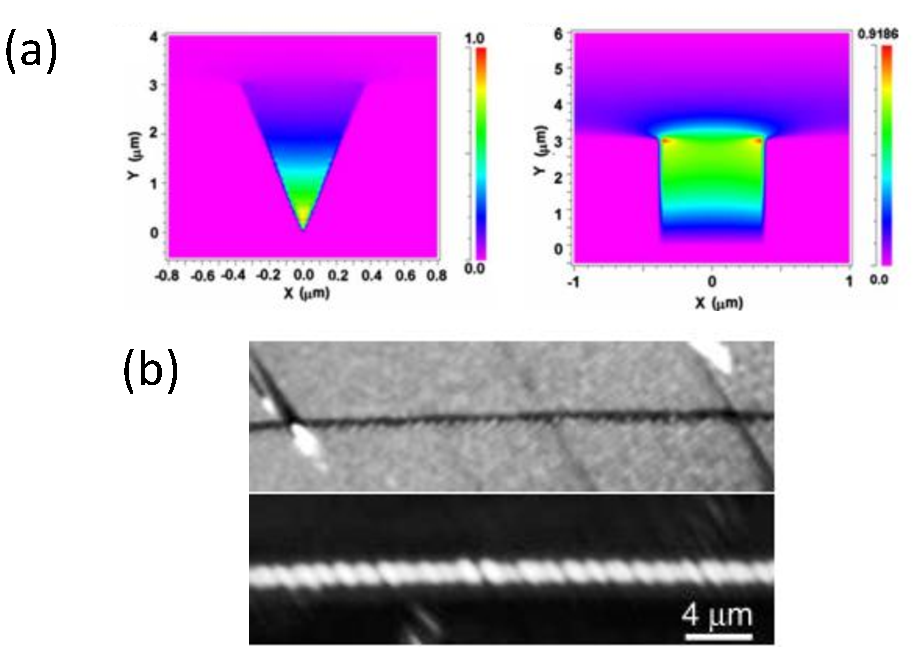
\includegraphics[width=0.6\textwidth]{Fig6}
\caption{(a) $E$-field profiles of channel plasmon polariton modes in a V-shaped (left) and trench (right) Au groove, with width 3.75\,$\mu$m and depth 3\,$\mu$m filled with air. (b) Topographical (top) and near-field optical (bottom) images for V-shaped Au slit with width 0.6\,$\mu$m and depth 1\,$\mu$m at $\lambda=1440$\,nm. Reproduced from Refs.\,\cite{Srivastava2009, Bozhevolnyi2005}.}
\label{3Fig6}
\end{figure} 

\section{Localised surface plasmons}
\subsection{Quasi-static approximation}
For spherical nanoparticles (NPs), if the diameter $d\ll\labmda$, the phase of the $E$-field is approximately constant across the particle, and we can solve the simplified problem of a sphere in an electrostatic field and include the harmonic time dependence of the field at the end. The geometry is shown in Fig.\,\ref{3Fig7}(a), with a homogeneous metal particle of diameter $d$ at the origin inside a dielectric medium, and $\vec{E_0} = E_0\vec{z}$. Solving the Laplace equation for the potential $\Phi$ ($\vec{E} = -\nabla\Phi$), we find
\begin{subequations}
\label{NPlaplace}
\begin{align}
\Phi_{in} &= -\frac{3\epsilon_d}{\epsilon_m+2\epsilon_d}E_0r\cos\theta \label{PhiIn}\\
\Phi_{out} &= -E_0r\cos\theta+\frac{\epsilon_m-\epsilon_d}{\epsilon_m+2\epsilon_d}E_0\left(\frac{d}{2}\right)^3\frac{\cos\theta}{r^2} \label{PhiOut}
\end{align}
\end{subequations}
at a distance $r$ from the centre of the sphere, where $\Phi_{in}$ and $\Phi_{out}$ represent the potentials inside and outside the sphere respectively. Note Eq.\,\ref{PhiOut} appears to be the superposition of the applied field $E_0$ and that of a dipole located at the origin. In this case we can see that the applied field induces a dipole moment $\vec{p}$ in the NP, and also introduce the polarisability $\alpha$ such that
\begin{subequations}
\label{NPdipole}
\begin{align}
\vec{p} &=4\pi\epsilon_0\epsilon_d\left(\frac{d}{2}\right)^3\frac{\epsilon_m-\epsilon_d}{\epsilon_m+2\epsilon_d}\vec{E_0} \label{NPmoment}\\
\alpha &= 4\pi\left(\frac{d}{2}\right)^3\frac{\epsilon_m-\epsilon_d}{\epsilon_m+2\epsilon_d} \label{NPpolarisability} .
\end{align}
\end{subequations}
A resonance in $\alpha$ is achieved when 
\begin{equation}
\centering
\epsilon_m(\omega) = -2\epsilon_d(\omega) ,
\label{Frolich}
\end{equation}
known as the Fr\"{o}lich condition, and provides the resonance frequency of the dipole LSP for a metallic NP. For a free electron gas in air, this condition is achieved at $\omega = \frac{\omega_0}{\sqrt{3}}$, but as can be seen from Eq.\,\ref{Frolich} the position is very sensitive to the dielectric environment around the particle. If harmonic time independece is included, we can see the resonance is caused by an oscillation of electrons in the NP, and as such causes a large field enhancement around the vicinity of the particle [Fig.\,\ref{3Fig7}(b)]. The LSP resonance also depends on the dielectric function of the metal, and for the same $d$ the Ag resonance is always higher in energy than Au [Fig.\,\ref{3Fig7}(c)]. Note also the asymmetric shape of the Au Np extinction, which is due to the onset of interband transitions in Au. For arrays of NPs, the resonance frequency in optical spectra is the same as single NPs if the particles are separated by more than $\approx2d$ \cite{Rechberger2003}.
\begin{figure}[ht] 
\centering    
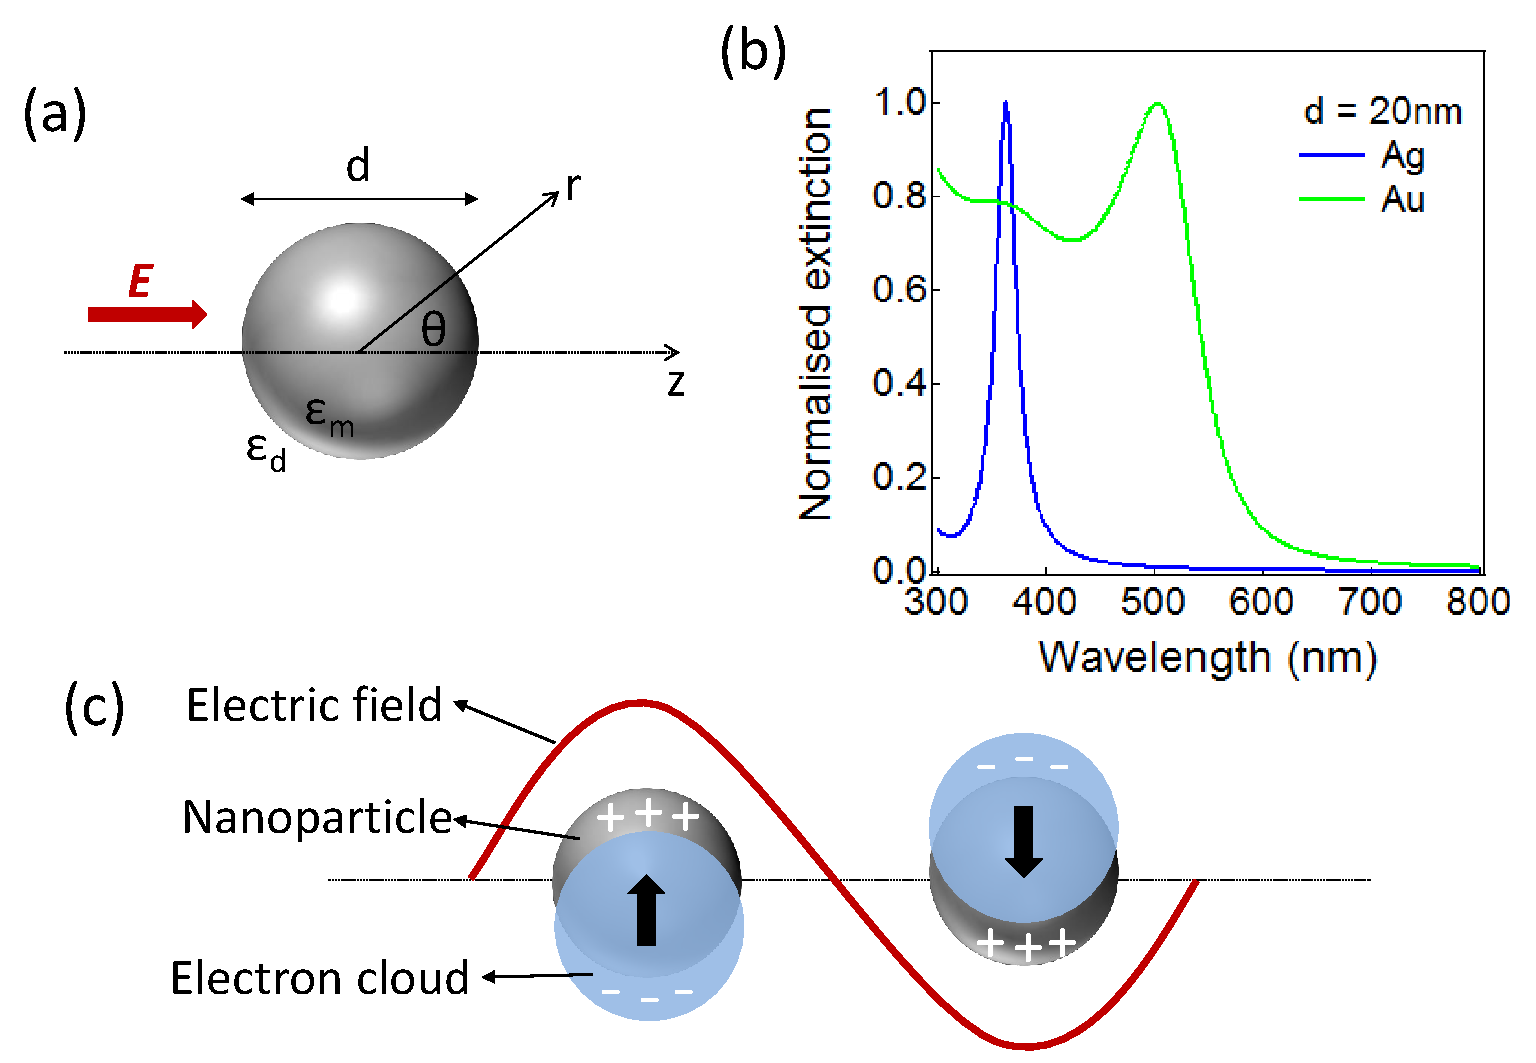
\includegraphics[width=\textwidth]{Fig7}
\caption{(a) Geometry of homogeneous metal sphere with diameter $d$ placed inside a electrostatic $E$-field. (b) $E$-field profile of dipole LSP. (c) Normalised extinction spectra for $d=20$\,nm Ag/Au NPs in air.}
\label{3Fig7}
\end{figure} 

The oscillating NP dipole leads to radiation, and can be seen as the scattering of light from the NP. The maximum in polarisability also leads to a resonant enhancement of the scattering $C_{\mathit{scat}}$ and absorption $C_{\mathit{abs}}$ cross section of the particle
\begin{subequations}
\label{NPcrossSections}
\begin{align}
C_{\mathit{scat}} &= \frac{k^4}{6\pi}|\alpha|^2 = \frac{8\pi}{3}k^4\left(\frac{d}{2}\right)^6 \left|\frac{\epsilon_m-\epsilon_d}{\epsilon_m+2\epsilon_d}\right|^2 \label{Scat}\\
C_{\mathit{abs}} &= k\textrm{Im}[\alpha] = 4\pik\left(\frac{d}{2}\right)^3\textrm{Im}\left[\frac{\epsilon_m-\epsilon_d}{\epsilon_m+2\epsilon_d}\right] \label{abs} ,
\end{align}
\end{subequations}
and we define extinction $C_{\mathit{ext}} = C_{\mathit{scat}}+C_{\mathit{abs}}$. For very small NPs absorption dominates over scattering due to its $d^3$ dependence, for example for $d=30$\,nm Ag NPs the extinction is almost entirely due to absorption [Fig.\,\ref{3Fig8}], while the reverse is true for $d=90$\,nm.
\begin{figure}[ht] 
\centering    
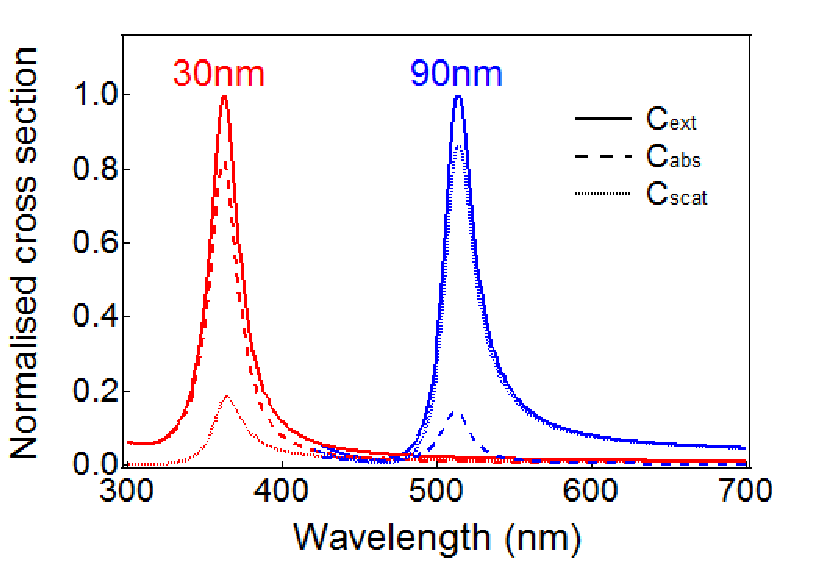
\includegraphics[width=0.6\textwidth]{Fig8}
\caption{Absorption (dashed lines), scattering (dotted lines) and extinction (solid lines) cross sections for Ag NPs $d=30$ and 90\,nm at $\lambda=500$\,nm in air according to Eq.\,\ref{NPcrossSections}, normalised so that the peak extinction is 1. The $d=90$\,nm data has been shifted for clarity.}
\label{3Fig8}
\end{figure}

\subsection{Size and shape effects}
The quasi-static approximation models the NP as an electric dipole whose resonance frequency depends purely on the relative dielectric functions of the metal and surrounding medium. The underlying assumption that the phase of the $E$-field across the particle is constant is only true for very small particles, and works well for $d<50$\,nm Ag particles [Fig.\,\ref{3Fig9}]. For larger particles an electrodynamic must be used, for example Mie theory \cite{Maier2007,} [CHECK BORN & WOLF], where the $E$-field waves are expanded into a superposition of partial waves (normal modes) that are spherical harmonics/radial components of Hertz vectors, and boundary conditions are used to find the absorption and scattering coefficients required. The normal modes are used in order to solve Maxwell's equations for a sphere interacting with an incoming plane wave. This method produces the redshift in LSP dipole resonance with $d$ as seen in experiment [Fig.\,\ref{3Fig9}], and also shows the emergence of higher order multipole modes for large particles. For example in Ag particles, a quadrupole mode can be excited and is first observed as a shoulder in the extinction spectrum for $d=90$\,nm.
\begin{figure}[ht] 
\centering    
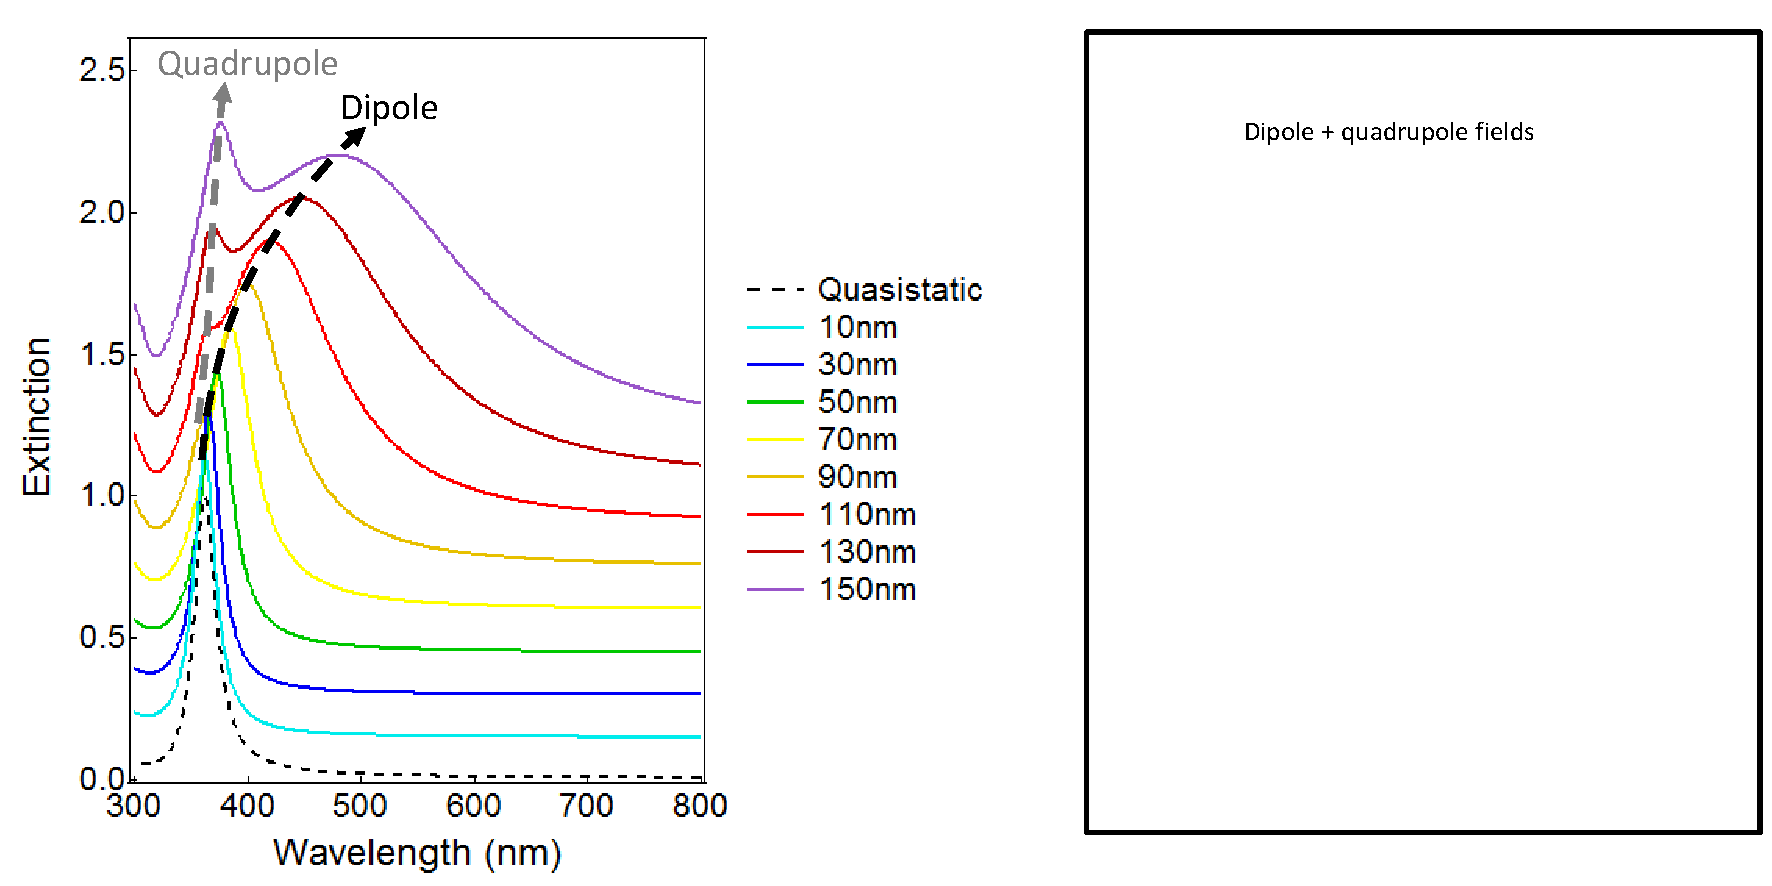
\includegraphics[width=0.6\textwidth]{Fig9}
\caption{Extinction for NPs with labelled $d$ in air using Mie theory, normalised to the dipole maximum and offset for clarity. The quasi-static approximation resonance is added for comparison.}
\label{3Fig9}
\end{figure}

The resonance of NPs is also very sensitive to the shape of the particle, and both quasi-static and Mie theory calculations can be adapted to the boundary conditions of non-spherical geometry. This provides great tunability to the LSP resonances via controlling of particle shape. Deviations from spherical geometry leads to the production of multiple redshifted peaks [Fig.\,\ref{3Fig10}(a)]. In the case of nanorods, we observe two LSP resonance in the spectra for unpolarised light: a transverse mode associated with electron oscillations along the short axis, and a longitudinal mode related to electron oscillations along the long axis, the resonance of which depends on the aspect ratio of the nanorod [Fig.\,\ref{3Fig10}(b)]. Therefore the longitudinal resonance can be tuned through a large range of the electromagnetic spectrum via the growth and assembly of such nanorods \cite{Wiley2006, Wiley2007, Chen2013}.
\begin{figure}[ht] 
\centering    
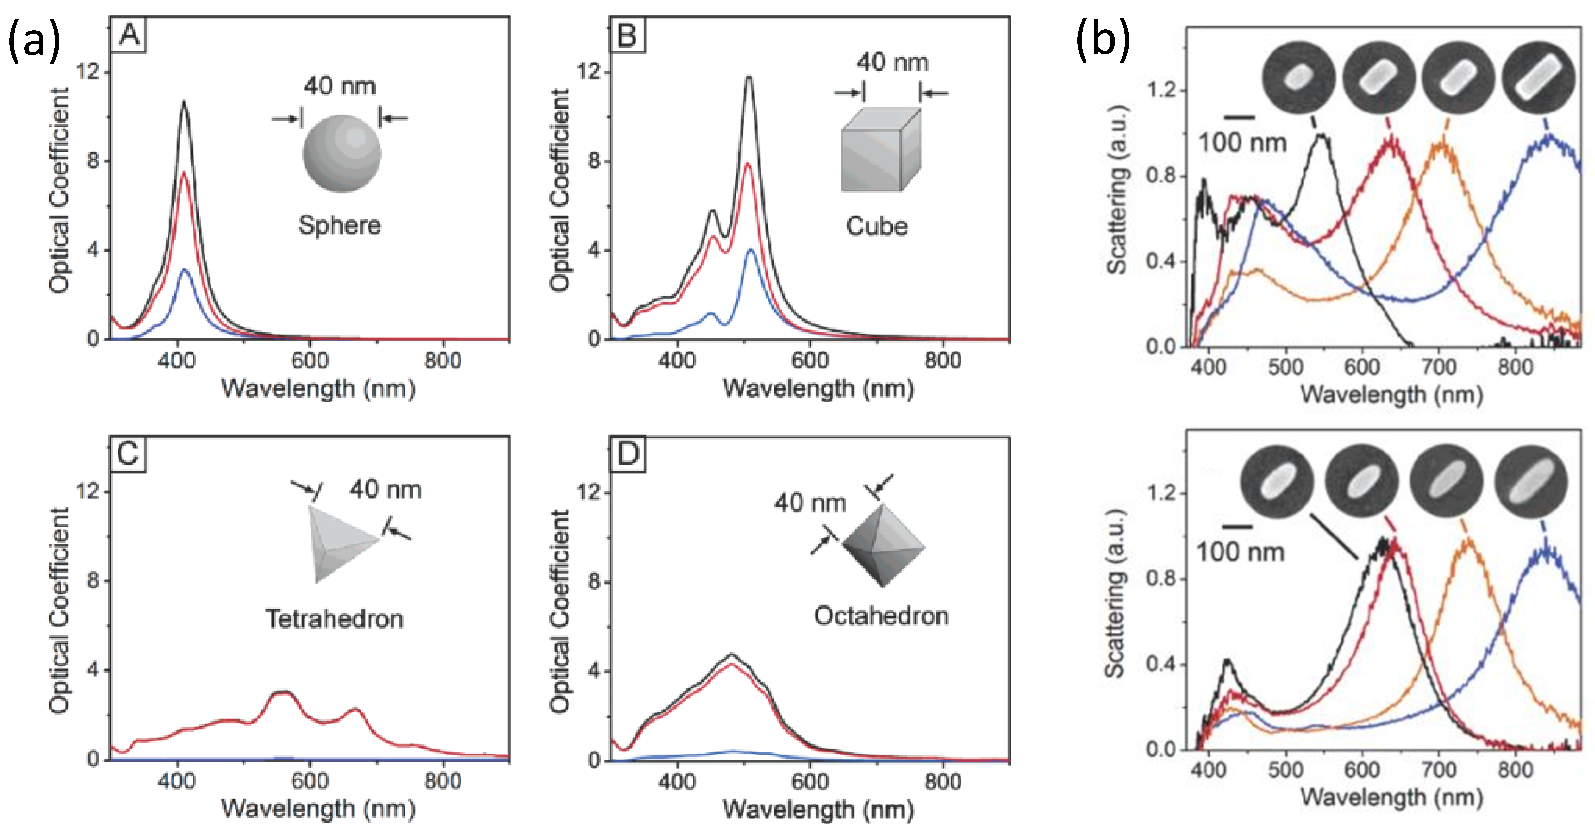
\includegraphics[width=0.8\textwidth]{Fig10}
\caption{(a) Discrete dipole approximation calculations of the extinction (black), absorption (red) and scattering (blue) of Ag nanoparticles with the geometries shown. (b) SEM images and normalised scattering spectra of individual Ag nanobar (top) nanorice (bottom) structures. Reproduced from Refs.\,\cite{Wiley2006, Wiley2007}.}
\label{3Fig10}
\end{figure}

\section{Conclusions}
Surface plasmons are collective oscillations of electrons in a metal. Such oscillations show resonant in many geometries, either guided in 2D structure such as planar metal films, or localised 0D nanoparticles. The resonance frequency depends on the relative dielectric functions of the metal and surrounding dielectric, and is very sensitive to the geomtry of the nanostructure. Surface plasmons cause large electric field enhancement around the vicinity of the metal, and can thus be used as a sensor. In periodic nanostructures, zone-folding allows incoming/outgoing light to reach parts of the plasmonic dispersion that may not be accessible otherwise, and the interaction between electrons and photons gives rise to many possible modes.